\documentclass[10pt, aspectratio=169, handout]{beamer}
\usefonttheme{professionalfonts}

\mode<presentation>{
  \usetheme{Berkeley}
  \usecolortheme{beaver}
  \usefonttheme{default}
  \setbeamertemplate{navigation symbols}{}
  \setbeamertemplate{caption}[numbered]
}

\setbeamertemplate{footline}{%
  \leavevmode%
  \hbox{%
    \begin{beamercolorbox}[wd=.85\paperwidth,ht=2.5ex,dp=1ex,left]{author in head/foot}%
      \usebeamerfont{author in head/foot}Digital Signal Processing, Fall 2025%
    \end{beamercolorbox}%
    \begin{beamercolorbox}[wd=.15\paperwidth,ht=2.5ex,dp=1ex,right]{date in head/foot}%
      \hspace*{0.5em}\insertframenumber{} / \inserttotalframenumber\hspace*{0.5em}%
    \end{beamercolorbox}%
  }%
  \vskip0pt%
}

\usepackage[english]{babel}
\usepackage[utf8]{inputenc}
\usepackage{tikz}
\usepackage{pgfplots}
\usepgfplotslibrary{groupplots}
\usetikzlibrary{calc, positioning, arrows.meta, backgrounds, pgfplots.groupplots, plotmarks}
\pgfplotsset{compat=newest}

\usepackage{array}
\usepackage{makecell}
\usepackage{verbatim}
\usepackage{graphicx}
\usepackage{amsfonts}
\usepackage{amsmath}
\usepackage{bm}
\usepackage{epstopdf}
\usepackage[absolute,overlay]{textpos}
\usepackage{hyperref}
\hypersetup{colorlinks=true, linkcolor=blue, urlcolor=cyan}

\title[ECEN 463/863]{Changing the Sampling Rate: Upsampling (Interpolation)}
\author{Maxx Seminario}
\institute{University of Nebraska-Lincoln}
\date{Fall 2025}

\begin{document}

%--------------------------------------------------
\begin{frame}
  \titlepage
\end{frame}

%--------------------------------------------------
\section{Motivation and Definitions}

\begin{frame}{Motivation for Upsampling}
\small
\textbf{Why increase the sampling rate?}
\begin{itemize}
  \item Interface between systems running at different sample rates (audio, telecom, sensors).
  \item Enable finer time resolution for subsequent processing (filtering, D/A conversion).
\end{itemize}

\vspace{0.25cm}
\textbf{Goal:} Given samples \(x[n] = x_c(nT)\), produce samples
\[
x_i[n] = x_c(nT_i), \qquad T_i = \frac{T}{L}
\]
so that the new sampling rate is \(L\) times larger.

\vspace{0.25cm}
\textbf{Definition (Upsampling / Interpolation):}
\[
x_i[n] = x\!\left[\frac{n}{L}\right] = x_c\!\left(\frac{nT}{L}\right), \quad n = 0, \pm L, \pm 2L, \dots
\]

\textbf{Problem:} Need the ``missing'' samples while preserving bandlimited structure.

\textbf{Solution Outline:}
\begin{enumerate}
  \item Insert "new samples" (expander) within the sequence.
  \item Lowpass filter with appropriate gain and cutoff to reconstruct intermediate samples.
\end{enumerate}
\end{frame}

%--------------------------------------------------
\begin{frame}{Expander and Interpolator Structure}
\small
\textbf{Expander (Sampling Rate Expander):}
\[
x_e[n] = \begin{cases}
x[n/L], & n = 0, \pm L, \pm 2L, \dots \\
0, & \text{otherwise}
\end{cases}
\quad \Longleftrightarrow \quad x_e[n] = \displaystyle \sum_{k=-\infty}^{\infty} x[k]\, \delta[n - kL]
\]

\textbf{Interpolator:} Lowpass filter \(h_i[n]\) (gain \(L\), cutoff \(\pi/L\)) applied to \(x_e[n]\):
\[
x_i[n] = (h_i * x_e)[n]
\]

\vspace{0.3cm}
\textbf{System Diagram:}
\begin{center}
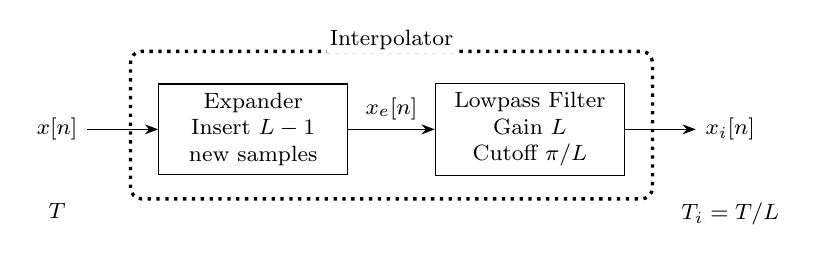
\begin{tikzpicture}[>=Stealth, node distance=0.9cm, every node/.style={font=\footnotesize}]
  \tikzset{block/.style={draw, minimum width=2.4cm, minimum height=1.0cm, align=center}}
  \node (xn) {$x[n]$};
  \node[block, right=0.9cm of xn] (expand) {Expander\\Insert $L-1$ \\ new samples};
  \node[block, right=1.1cm of expand] (lpf) {Lowpass Filter\\Gain $L$\\Cutoff $\pi/L$};
  \node (xin) [right=0.9cm of lpf] {$x_i[n]$};

  \draw[->] (xn.east) -- (expand.west);
  \draw[->] (expand.east) -- node[midway, above] {$x_e[n]$} (lpf.west);
  \draw[->] (lpf.east) -- (xin.west);

  \node[below=0.55cm of xn] {$T$};
  \node[below=0.55cm of xin] {$T_i = T/L$};

  % Dotted outline around the interpolator (Expander + Lowpass Filter)
  \coordinate (boxSW) at ($(expand.south west)+(-0.35,-0.30)$);
  \coordinate (boxNE) at ($(lpf.north east)+(0.35,0.40)$);
  \draw[dotted, very thick, rounded corners] (boxSW) rectangle (boxNE);

  % Label ABOVE the dotted outline (top-center)
  \path let \p1=(boxSW), \p2=(boxNE) in coordinate (boxTopCenter) at ({(\x1+\x2)/2}, {\y2});
  \node[font=\footnotesize, fill=white, inner sep=1pt] at ([yshift=4pt]boxTopCenter) {Interpolator};
\end{tikzpicture}
\end{center}

\textbf{Terminology:} Expander + Antialias (Interpolation) Filter = \textbf{Interpolator}.
\end{frame}

%--------------------------------------------------
% Frame 1: Compute the DTFT of x_e[n]
\begin{frame}{Frequency-Domain Effect of Expansion: DTFT of $x_e[n]$}
\small
\textbf{Expander definition:}
\[
x_e[n] =
\begin{cases}
x[n/L], & n = 0, \pm L, \pm 2L, \dots \\
0, & \text{otherwise}
\end{cases}
\quad \Longleftrightarrow \quad
x_e[n] = \displaystyle \sum_{k=-\infty}^{\infty} x[k]\,\delta[n-kL]
\]

\textbf{Compute the DTFT of $x_e[n]$:}
\[
\begin{aligned}
X_e(e^{j\omega})
&= \sum_{n=-\infty}^{\infty} x_e[n]\; e^{-j\omega n} \\
&= \sum_{n=-\infty}^{\infty} \left(\sum_{k=-\infty}^{\infty} x[k]\,\delta[n-kL]\right) e^{-j\omega n} \\
&= \sum_{k=-\infty}^{\infty} x[k]\; e^{-j\omega (kL)} \\
&= \sum_{k=-\infty}^{\infty} x[k]\; e^{-j(\omega L) k} \\
&= X(e^{j\,\omega L})
\end{aligned}
\]

\textbf{Key result:}
\[
\boxed{\,X_e(e^{j\omega}) = X(e^{j\omega L})\,}
\]

\textbf{Immediate consequence:} The frequency variable is scaled by $L$ (i.e., the baseband spectrum appears compressed by $L$ in $X_e$).
\end{frame}

% Frame 2: Interpretation and interpolation filter
\begin{frame}{Frequency-Domain Effect of Expansion: Interpretation and Filter}
\small
\textbf{Result:}
\[
X_e(e^{j\omega}) = X(e^{j\omega L})
\]

\textbf{Interpretation:}
\begin{itemize}
  \item Baseband spectrum is \textbf{compressed} by factor $L$.
  \item Multiple frequency-scaled images appear within $|\omega|\le\pi$ due to DTFT periodicity.
  \item An interpolation lowpass (cutoff $\pi/L$) removes images and rescales amplitude.
\end{itemize}

\textbf{Interpolator output:}
\[
X_i(e^{j\omega}) = H_i(e^{j\omega})\,X_e(e^{j\omega}) \approx X(e^{j\omega}) \quad (\text{ideal})
\]

\textbf{Ideal interpolation filter:}
\[
H_i(e^{j\omega}) =
\begin{cases}
L, & |\omega|\le \pi/L \\
0, & \pi/L < |\omega|\le \pi
\end{cases}
\]

\textbf{Gain justification:} Scale by $L$ so spectral amplitude matches new sampling rate:
\[
L \cdot \frac{1}{T} \;=\; \frac{1}{T/L} \;=\; \frac{1}{T_i}.
\]
\end{frame}

%--------------------------------------------------

\begin{frame}{Downsampling with Aliasing - Frequency Domain}
\small

\begin{center}
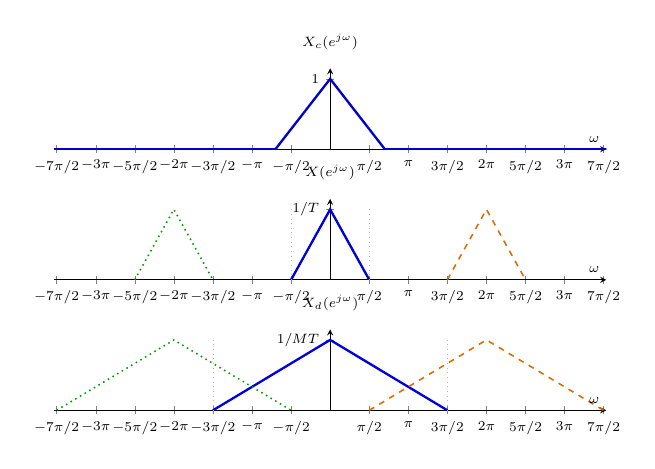
\begin{tikzpicture}[scale=0.7]
  \begin{groupplot}[
    group style={group size=1 by 3, vertical sep=0.9cm},
    width=11.6cm,
    height=3.05cm,
    axis lines=middle,
    xmin=-11.1, xmax=11.1,
    ymin=0, ymax=1.15,
    tick label style={font=\scriptsize},
    label style={font=\scriptsize},
    title style={font=\scriptsize},
    xtick={-10.9956,-9.4248,-7.85398,-6.2832,-4.7124,-3.1416,-1.5708,0,1.5708,3.1416,4.7124,6.2832,7.85398,9.4248,10.9956},
    xticklabels={$-7\pi/2$,$-3\pi$,$-5\pi/2$,$-2\pi$,$-3\pi/2$,$-\pi$,$-\pi/2$,$0$,$\pi/2$,$\pi$,$3\pi/2$,$2\pi$,$5\pi/2$,$3\pi$,$7\pi/2$},
    xlabel={$\omega$}
  ]

  %------------------------------------------------------
  % Plot 1: Original spectrum with endpoints at ±Ω_N (numeric y tick 1)
  %------------------------------------------------------
  \def\OmegaN{2.2}
  \nextgroupplot[
    title={$X_c(e^{j\omega})$},
    ytick={0,1},
    yticklabels={$0$,$1$}
  ]
  \addplot[blue!80!black, very thick] coordinates {
    (-11.1,0) (-\OmegaN,0) (0,1) (\OmegaN,0) (11.1,0)
  };
  \node[red!70!black, font=\scriptsize, anchor=north east] at (axis cs:-\OmegaN,0) {$-\Omega_N$};
  \node[red!70!black, font=\scriptsize, anchor=north west] at (axis cs:\OmegaN,0) {$+\Omega_N$};
  \node[blue!60!black, font=\scriptsize] at (axis cs:0,-0.23) {Bandwidth extends to $\pm\Omega_N$};

  %------------------------------------------------------
  % Plot 2: Narrow central triangle and narrow alias replicas at ±2π (peak labeled 1/T)
  %------------------------------------------------------
  \nextgroupplot[
    title={$X(e^{j\omega})$},
    ytick={0,1},
    yticklabels={$0$,$1/T$}
  ]
  % Central narrow triangle: support [-π/2, π/2]
  \addplot[blue!85!black, very thick]
    coordinates {(-1.5708,0) (0,1) (1.5708,0)};
  % Narrow replica at +2π: support [3π/2,5π/2] = [4.7124,7.85398]
  \addplot[orange!85!black, thick, dashed]
    coordinates {(4.7124,0) (6.2832,1) (7.85398,0)};
  % Narrow replica at -2π: support [-5π/2,-3π/2] = [-7.85398,-4.7124]
  \addplot[green!60!black, thick, dotted]
    coordinates {(-7.85398,0) (-6.2832,1) (-4.7124,0)};
  % Vertical guides for narrow central triangle
  \draw[gray!55,dotted] (axis cs:-1.5708,0) -- (axis cs:-1.5708,1.05);
  \draw[gray!55,dotted] (axis cs: 1.5708,0) -- (axis cs: 1.5708,1.05);
  \node[red!70!black, font=\scriptsize] at (axis cs:0,-0.25) {Narrow replicas shown individually};

  %------------------------------------------------------
  % Plot 3: Wide triangles (width 3π) centered at 0, ±2π (peak labeled 1/T)
  %------------------------------------------------------
  \nextgroupplot[
    title={$X_d(e^{j\omega})$},
    ytick={0,1},
    yticklabels={$0$,$1/MT$}
  ]
  % Central wide triangle: support [-3π/2, 3π/2] = [-4.7124,4.7124]
  \addplot[blue!85!black, very thick]
    coordinates {(-4.7124,0) (0,1) (4.7124,0)};
  % Wide replica at +2π: center 2π; support [2π-3π/2, 2π+3π/2] = [π/2, 7π/2] = [1.5708,10.9956]
  \addplot[orange!85!black, thick, dashed]
    coordinates {(1.5708,0) (6.2832,1) (10.9956,0)};
  % Wide replica at -2π: support [-2π-3π/2, -2π+3π/2] = [-7π/2, -π/2] = [-10.9956,-1.5708]
  \addplot[green!60!black, thick, dotted]
    coordinates {(-10.9956,0) (-6.2832,1) (-1.5708,0)};
  % Vertical guides for central wide triangle edges
  \draw[gray!55,dotted] (axis cs:-4.7124,0) -- (axis cs:-4.7124,1.05);
  \draw[gray!55,dotted] (axis cs: 4.7124,0) -- (axis cs: 4.7124,1.05);
  \node[purple!70!black, font=\scriptsize] at (axis cs:0,-0.25) {Wide replicas (same shape) centered at shifts};

  \end{groupplot}
\end{tikzpicture}
\end{center}

% \textbf{Note:} Third plot illustrates a larger bandwidth case (each replica width $3\pi$) still centered at $0,\pm 2\pi$; all shapes are individual (no summation).
\end{frame}

%--------------------------------------------------

\begin{frame}{Downsampling with Anti Aliasing - Frequency Domain}
\small

% Note: Updated SECOND plot per request:
%   Each replica (centered at -2\pi, 0, 2\pi) is now a composite "pedestal + peak":
%   A rectangle (constant pedestal amplitude A) spanning local window edges (±\pi/3 around its center),
%   with a triangular cap rising to a higher peak at the replica center.
%   Vertical lines drawn at the window cutoff frequencies (±\pi/3 for the central, shifted for outer replicas).
%   Outside those window edges the signal is zero.
% Adjust pedestal height via \RectH and peak height via 1/T (symbolic).
\def\RectH{0.35} % pedestal fraction of peak (change if desired)

\begin{center}
\begin{tikzpicture}[scale=0.7]
  \begin{groupplot}[
    group style={group size=1 by 3, vertical sep=1.2cm},
    width=11.6cm,
    height=3.05cm,
    axis lines=middle,
    xmin=-11.1, xmax=11.1,
    ymin=0, ymax=1.15,
    tick label style={font=\scriptsize},
    label style={font=\scriptsize},
    title style={font=\scriptsize},
    xtick={-10.9956,-9.4248,-7.85398,-6.2832,-4.7124,-3.1416,-1.5708,0,1.5708,3.1416,4.7124,6.2832,7.85398,9.4248,10.9956},
    xticklabels={$-7\pi/2$,$-3\pi$,$-5\pi/2$,$-2\pi$,$-3\pi/2$,$-\pi$,$-\pi/2$,$0$,$\pi/2$,$\pi$,$3\pi/2$,$2\pi$,$5\pi/2$,$3\pi$,$7\pi/2$},
    xlabel={$\omega$}
  ]

  %------------------------------------------------------
  % Plot 1: Original spectrum with endpoints at ±Ω_N (numeric y tick 1)
  %------------------------------------------------------
  \def\OmegaN{2.2}
  \nextgroupplot[
    title={$X_c(e^{j\omega})$},
    ytick={0,1},
    yticklabels={$0$,$1$}
  ]
  \addplot[blue!80!black, very thick] coordinates {
    (-11.1,0) (-\OmegaN,0) (0,1) (\OmegaN,0) (11.1,0)
  };
  \node[red!70!black, font=\scriptsize, anchor=north east] at (axis cs:-\OmegaN,0) {$-\Omega_N$};
  \node[red!70!black, font=\scriptsize, anchor=north west] at (axis cs:\OmegaN,0) {$+\Omega_N$};
  \node[blue!60!black, font=\scriptsize] at (axis cs:0,-0.23) {Bandwidth extends to $\pm\Omega_N$};

  %------------------------------------------------------
  % Plot 2: Windowed replicas with pedestal + peak (rectangle with triangle on top)
  % Central window edges at ±\pi/3; outer windows shifted by ±2\pi.
  %------------------------------------------------------
  \nextgroupplot[
    title={$X_{\text{windowed}}(e^{j\omega})$ (Window $|\omega-\omega_0|\le \pi/3$)},
    ytick={0,1},
    yticklabels={$0$,$1/T$}
  ]
  % Constants:
  % pi/3 = 1.0472 ; 2pi = 6.2832
  % Outer edges: center ±2π ± π/3 = ±(2π ± π/3)
  % Pedestal + triangle outlines given as single polygon each.
  % Central composite shape:
  \addplot[blue!85!black, very thick]
    coordinates {
      (-1.0472,0) (-1.0472,\RectH) (0,1) (1.0472,\RectH) (1.0472,0)
    };
  % Right composite shape (shifted +2π):
  \addplot[orange!85!black, thick, dashed]
    coordinates {
      (6.2832-1.0472,0) (6.2832-1.0472,\RectH) (6.2832,1) (6.2832+1.0472,\RectH) (6.2832+1.0472,0)
    };
  % Left composite shape (shifted -2π):
  \addplot[green!60!black, thick, dotted]
    coordinates {
      (-6.2832-1.0472,0) (-6.2832-1.0472,\RectH) (-6.2832,1) (-6.2832+1.0472,\RectH) (-6.2832+1.0472,0)
    };

  % Vertical window cutoff lines (central)
  \draw[gray!55,dotted] (axis cs:-1.0472,0) -- (axis cs:-1.0472,1.05);
  \draw[gray!55,dotted] (axis cs: 1.0472,0) -- (axis cs: 1.0472,1.05);
  % Vertical window cutoff lines (right)
  \draw[gray!55,dotted] (axis cs:6.2832-1.0472,0) -- (axis cs:6.2832-1.0472,1.05);
  \draw[gray!55,dotted] (axis cs:6.2832+1.0472,0) -- (axis cs:6.2832+1.0472,1.05);
  % Vertical window cutoff lines (left)
  \draw[gray!55,dotted] (axis cs:-6.2832-1.0472,0) -- (axis cs:-6.2832-1.0472,1.05);
  \draw[gray!55,dotted] (axis cs:-6.2832+1.0472,0) -- (axis cs:-6.2832+1.0472,1.05);

  \node[red!70!black, font=\scriptsize] at (axis cs:0,-0.25) {Outside each window ($|\omega-\omega_0|>\pi/3$) zeroed};

  %------------------------------------------------------
  % Plot 3: Wide triangles (unchanged)
  %------------------------------------------------------
  \nextgroupplot[
    title={$X_d(e^{j\omega})$},
    ytick={0,1},
    yticklabels={$0$,$1/MT$}
  ]

  % Width now = 2π (half-width π). Numerical: π = 3.1416
  % Centers remain at 0, +2π (6.2832), -2π (-6.2832).
  % Edges:
  %   Central: -π .. +π  => -3.1416 .. 3.1416
  %   Right:   2π-π .. 2π+π  => 3.1416 .. 9.4248
  %   Left:   -2π-π .. -2π+π => -9.4248 .. -3.1416

  % Central composite shape (rectangle + triangle)
  \addplot[blue!85!black, very thick]
    coordinates {
      (-3.1416,0) (-3.1416,\RectH) (0,1) (3.1416,\RectH) (3.1416,0)
    };

  % Right composite shape (center +2π)
  \addplot[orange!85!black, thick, dashed]
    coordinates {
      (3.1416,0) (3.1416,\RectH) (6.2832,1) (9.4248,\RectH) (9.4248,0)
    };

  % Left composite shape (center -2π)
  \addplot[green!60!black, thick, dotted]
    coordinates {
      (-9.4248,0) (-9.4248,\RectH) (-6.2832,1) (-3.1416,\RectH) (-3.1416,0)
    };

  % Vertical boundary lines at all shape edges
  \draw[gray!55,dotted] (axis cs:-3.1416,0) -- (axis cs:-3.1416,1.05);
  \draw[gray!55,dotted] (axis cs: 3.1416,0) -- (axis cs: 3.1416,1.05);
  \draw[gray!55,dotted] (axis cs:-9.4248,0) -- (axis cs:-9.4248,1.05);
  \draw[gray!55,dotted] (axis cs:-3.1416,0) -- (axis cs:-3.1416,1.05);
  \draw[gray!55,dotted] (axis cs: 3.1416,0) -- (axis cs: 3.1416,1.05);
  \draw[gray!55,dotted] (axis cs: 9.4248,0) -- (axis cs: 9.4248,1.05);
  \end{groupplot}
\end{tikzpicture}
\end{center}

\end{frame}

%--------------------------------------------------
\begin{frame}{Interpolation Filter Impulse Response}
\small
Ideal lowpass interpolation filter (\(L\)-fold upsampling):
\[
H_i(e^{j\omega}) =
\begin{cases}
L, & |\omega|\le \pi/L \\
0, & \pi/L < |\omega|\le \pi
\end{cases}
\]

Impulse response (sinc form):
\[
h_i[n] = \frac{\sin(\pi n / L)}{\pi n / L}
\]

\textbf{Key Properties:}
\begin{itemize}
  \item \(h_i[0] = 1\).
  \item \(h_i[n] = 0\) for \(n = \pm L, \pm 2L, \dots\) (zeros at integer multiples of \(L\)).
  \item Acts like ideal reconstruction between the nonzero locations of \(x_e[n]\).
\end{itemize}

\textbf{Output Samples:}
\[
x_i[n] = \sum_{k=-\infty}^{\infty} x[k] \frac{\sin[\pi(n - kL)/L]}{\pi(n - kL)/L}
\]

For \(n = mL\) (multiples of \(L\)):
\[
x_i[mL] = x[m]
\]
(Perfect retention of existing samples.)
\end{frame}

%--------------------------------------------------
\begin{frame}{Derivation Recap}
\small
Starting with expander output:
\[
x_e[n] = \sum_{k=-\infty}^{\infty} x[k]\,\delta[n - kL]
\]

Filtering:
\[
x_i[n] = (h_i * x_e)[n] = \sum_{m=-\infty}^{\infty} h_i[n-m]\, x_e[m]
= \sum_{k=-\infty}^{\infty} h_i[n - kL]\, x[k]
\]

Using \(h_i[n]\) definition:
\[
x_i[n] = \sum_{k=-\infty}^{\infty} x[k] \frac{\sin\left(\pi (n - kL)/L\right)}{\pi (n - kL)/L}
\]

Matches continuous-time sampling at \(T_i = T/L\):
\[
x_i[n] = x_c(nT_i) = x_c\left(\frac{nT}{L}\right)
\]

\textbf{Conclusion:} Ideal \(L\)-fold interpolation exactly reconstructs bandlimited signal at higher rate.
\end{frame}

%--------------------------------------------------
\section{Examples}

\begin{frame}{Example: $L=3$ (Spectral View)}
\small
Assume original \(X(e^{j\omega})\) occupies \(|\omega| \le \pi/2\).

After expansion by \(L=3\):
\[
X_e(e^{j\omega}) = X(e^{j3\omega})
\]
Nonzero only for \(|\omega| \le \pi/6\) in principal lobe; other compressed images appear.

Interpolator \(H_i\):
\[
H_i(e^{j\omega}) = \begin{cases}
3, & |\omega| \le \pi/3 \\
0, & \pi/3 < |\omega| \le \pi
\end{cases}
\]

Result:
\[
X_i(e^{j\omega}) = H_i(e^{j\omega}) X_e(e^{j\omega}) \approx X(e^{j\omega})
\]

\textbf{Bandwidth Relation:} Needed cutoff \(\pi/3\) ensures only baseband compressed copy passes plus gain correction.
\end{frame}

%--------------------------------------------------
\begin{frame}{Numerical Example}
\small
Let \(x[n] = \cos(0.25\pi n)\), upsample by \(L=4\).

Zero-stuff:
\[
x_e[n] =
\begin{cases}
\cos(0.25\pi (n/4)), & n \equiv 0 \; (\text{mod } 4) \\
0, & \text{otherwise}
\end{cases}
= \begin{cases}
\cos(0.0625\pi n), & n = 0, \pm 4, \pm 8, \dots \\
0, & \text{else}
\end{cases}
\]

Filter with ideal interpolation \(h_i[n]\) (cutoff \(\pi/4\), gain 4) gives:
\[
x_i[n] = \cos(0.25\pi n) \quad \text{(now evaluated at finer grid)}
\]

\textbf{Energy / Amplitude:} Gain 4 compensates for zero insertion dilution.

\textbf{Practical:} Use finite-length FIR approximation of \(h_i[n]\) (windowed sinc) and polyphase decomposition for efficiency.
\end{frame}

%--------------------------------------------------
\section{Implementation Considerations}

\begin{frame}{Practical Interpolation Filter Design}
\small
\textbf{Ideal Filter Not Implementable:} Infinite-length sinc, noncausal.

\textbf{Design Approaches:}
\begin{itemize}
  \item Windowed-sinc FIR (Kaiser, Hamming) with cutoff \(\pi/L\).
  \item Parks–McClellan (equiripple) lowpass design specifying passband ripple and stopband attenuation.
  \item IIR filters (less common due to phase distortion concerns).
\end{itemize}

\textbf{Gain Handling:}
\begin{itemize}
  \item Include factor \(L\) inside filter taps.
  \item Or multiply output after filtering (less efficient).
\end{itemize}

\textbf{Performance Metrics:}
\begin{itemize}
  \item Passband ripple (affects amplitude accuracy of retained frequencies).
  \item Transition width (larger \(L\) often permits narrower filter).
  \item Stopband attenuation (controls interpolation imaging).
\end{itemize}
\end{frame}

%--------------------------------------------------
% \begin{frame}{Polyphase Implementation}
% \small
% \textbf{Motivation:} Direct zero-stuff + full-rate filtering wastes multiplications on zeros.

% \textbf{Polyphase Decomposition:}
% \[
% h_i[n] \rightarrow \{ e_0[n], e_1[n], \dots, e_{L-1}[n]\}
% \]
% so that
% \[
% y[n] = \sum_{r=0}^{L-1} e_r[n] * x\left[\frac{n - r}{L}\right]
% \]

% \textbf{Key Idea:}
% \begin{itemize}
%   \item Compute only one subfilter per output sample.
%   \item Throughput improved by factor \(L\).
% \end{itemize}

% \textbf{Applications:} High-quality sample rate converters, multistage interpolation (cascade small factors).

% \textbf{Benefit:} Lower computational load, better cache usage.
% \end{itemize}
% \end{frame}

%--------------------------------------------------
\begin{frame}{Alias and Imaging Considerations}
\small
\textbf{Assumption:} Original \(x[n]\) from alias-free sampling of bandlimited \(x_c(t)\).

\textbf{If Not Bandlimited:}
\begin{itemize}
  \item Interpolation filter will pass baseband AND distort edges.
  \item Imaging components (scaled copies) may leak if filter insufficient.
\end{itemize}

\textbf{Quality Factors:}
\begin{itemize}
  \item Stopband attenuation sets rejection of compressed images.
  \item Passband flatness ensures accurate amplitude of restored spectrum.
  \item Group delay linearity affects waveform shape (phase-sensitive applications).
\end{itemize}

\textbf{Preconditioning:} Sometimes mild lowpass applied before interpolation to suppress high-frequency noise.
\end{frame}

%--------------------------------------------------
\begin{frame}{Upsampling vs. Downsampling (Comparison)}
\small
\begin{itemize}
  \item \textbf{Downsampling:} Bandwidth must shrink (filter then decimate). Aliasing risk if not filtered.
  \item \textbf{Upsampling:} Bandwidth must remain limited; expansion creates \emph{images} requiring lowpass removal.
  \item \textbf{Filters:} Downsampling uses antialias filter (cutoff \(\pi/M\)). Upsampling uses interpolation filter (cutoff \(\pi/L\)).
  \item \textbf{Scaling:} Interpolation filter has gain \(L\); decimation filter usually unity gain in passband.
  \item \textbf{Artifacts:} Downsampling risk: aliasing; Upsampling risk: imaging.
\end{itemize}
\end{frame}

%--------------------------------------------------
\section{Summary}

\begin{frame}{Summary of Upsampling Concepts}
\small
\textbf{Core Steps:}
\[
x[n] \xrightarrow{\text{Insert } L-1 \text{ zeros}} x_e[n] \xrightarrow{h_i[n]} x_i[n]
\]

\textbf{Key Formula:}
\[
X_e(e^{j\omega}) = X(e^{j\omega L}), \qquad
H_i(e^{j\omega}) = \begin{cases} L, & |\omega|\le \pi/L \\ 0, & \text{else} \end{cases}
\]

\[
x_i[n] = \sum_{k=-\infty}^{\infty} x[k] \frac{\sin[\pi(n - kL)/L]}{\pi(n - kL)/L}
\]

\textbf{Conditions:}
\begin{itemize}
  \item Original sequence must be bandlimited (no alias in initial sampling).
  \item Interpolation filter approximates ideal lowpass.
\end{itemize}

\textbf{Design Notes:}
\begin{itemize}
  \item Use finite-length FIR (windowed-sinc) or polyphase structure.
  \item Gain normalization critical (factor \(L\)).
\end{itemize}

\textbf{Artifacts to Control:}
\begin{itemize}
  \item Imaging (spectral copies).
  \item Passband ripple and stopband attenuation.
\end{itemize}
\end{frame}

%--------------------------------------------------
\begin{frame}{Practical Interpolation Checklist}
\small
\textbf{Given:} Target upsampling factor \(L\).

\textbf{Checklist:}
\begin{enumerate}
  \item Confirm input bandlimit \(|\omega| \le \omega_B \le \pi\).
  \item Determine required cutoff: \(\omega_c = \min(\pi/L, \omega_B)\).
  \item Specify passband ripple (e.g. < 0.1 dB) and stopband attenuation (e.g. > 60 dB).
  \item Design FIR filter taps; include scaling by \(L\).
  \item Implement via polyphase (split taps into \(L\) subfilters).
  \item Validate amplitude and spectral suppression (FFT of output).
  \item (Optional) Multistage interpolation if \(L\) factor large (factorization).
\end{enumerate}

\textbf{Performance Tips:}
\begin{itemize}
  \item Larger \(L\) shrinks required passband, enabling shorter filters.
  \item Multistage: reduce overall tap count vs single sharp filter.
  \item Fixed-point: ensure sufficient headroom after gain \(L\).
\end{itemize}
\end{frame}

%--------------------------------------------------
\begin{frame}{Closing Remarks}
\small
\textbf{Upsampling (Interpolation)} is the discrete-time dual of:
\begin{itemize}
  \item D/C reconstruction (conceptually).
  \item Downsampling with antialias filter (role reversal of images vs aliases).
\end{itemize}

\textbf{Takeaways:}
\begin{itemize}
  \item Zero insertion alone distorts spectrum (images).
  \item Proper lowpass filter restores original bandwidth and amplitude.
  \item Exact reconstruction relies on original bandlimited assumption.
\end{itemize}

Next Lecture: \textit{Rational sampling-rate conversion} (cascade interpolate + decimate).
\end{frame}

\end{document}